\section{Auswertung}
\label{sec:Auswertung}
\subsection{Zählrohr-Charakteristik}
\label{subsec:Zählrohr-Charakteristik}
Die Charakteristik des Zählrohres wird anhand der Messergebnisse (siehe Tabelle \ref{tab:Messwerte}) in die Abbildung \ref{fig:Charakteristik} aufgenommen.
Der Plateau-Bereich wird von 390 bis 610 $\si{\volt}$ angenommen, somit ist der Bereich $\SI{280}{\volt}$ lang.
Mithilfe von ipython wird eine lineare Ausgleichsrechnung für den Plateau-Bereich durchgeführt.
Für die Ausgleichgerade ergibt sich:
\begin{equation*}
  N = (1.169 \pm 0.325)U + (9575.69 \pm 163.72)
\end{equation*}
Die Plateau-Steigung kann auch mit 101,22\% pro $\SI{100}{\volt}$ angegeben werden.
Eine geeignete Zählrohrspannung ist $\SI{400}{\volt}$, da diese etwas über der Spannung $U_\text{E}$ und im Auslösebereich liegt.
\begin{figure}
  \centering
  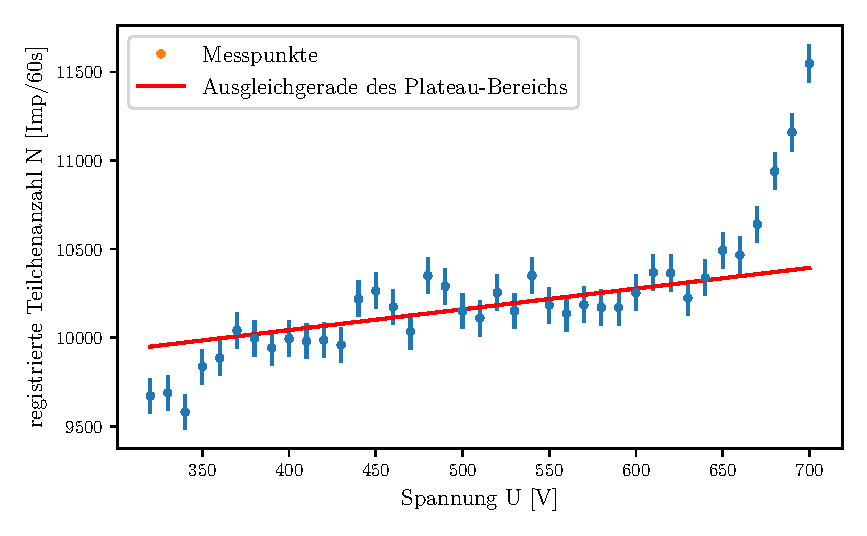
\includegraphics{Plateau_Gerade.pdf}
  \caption{Zählrohrcharakteristik mit Ausgleichgerade für den Plateau-Bereich.}
  \label{fig:Charakteristik}
\end{figure}

\subsection{Zeitlicher Abstand zwischen Primär- und Nachentladungsimpuls}
\label{subsec:Primär_Nachentladung}
Die Erholzeit kann nicht aus der Abbildung \ref{fig:Momentaufnahme} entnommen werden.
Dadurch entfällt diese Aufgabe.

\subsection{Bestimmung der Totzeit}
\label{subsec:Totzeit}

\subsubsection{Oszilloskop}
Anhand der Abbildung \ref{fig:Momentaufnahme} soll die Totzeit bestimmt werden.
Die Zeit zwischen dem ersten und zweitem Puls wird abgelesen und auf $\SI{100}{\micro\second}$ geschätzt.

\begin{figure}
  \centering
  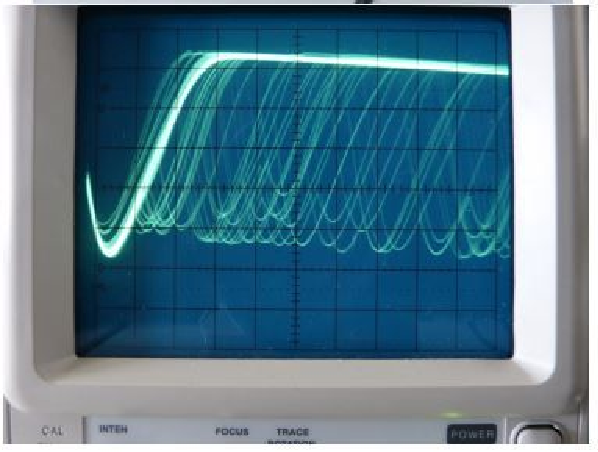
\includegraphics[width=\textwidth]{Momentaufnahme.pdf}
  \caption{Momentaufnahme der Anzeige des Oszilloskops.\cite{anleitung}}
  \label{fig:Momentaufnahme}
\end{figure}

\subsubsection{Zwei-Quellen-Methode}
Mit der Formel \eqref{eqn:totzeit} wird die Totzeit mit den folgenden Zählraten ermittelt:
\begin{align*}
  N_1 &= \frac{96041}{120} \text{Imp/s} \\
  N_{1+2} &= \frac{158479}{120} \text{Imp/s} \\
  N_2 &= \frac{76518}{120} \text{Imp/s} \\
\end{align*}
Für diese Messwerte wurde die Messzeit auf $\SI{120}{\second}$ erhöht, um eine genauere Messung durchzuführen.
Mit der Fehlerfortpflanzung nach Gauß folgt insgesamt für die Totzeit $T = \SI{115 \pm 0.047}{\micro\second}$.

\subsection{Freigesetzte Ladung pro einfallendem Teilchen}
\label{subsec:LadungProTeilchen}
Aus den Messwerten aus Tabelle \ref{tab:Messwerte} und der Formel \ref{eqn:Ladung} werden die Ladungen pro Teilchen bestimmt.
Die Ergebnisse sind in Tabelle \ref{tab:Ladungen} festgehalten.
Die dazugehörigen Messunsicherheiten wurden mit der Fehlerfortpflanzung nach Gauß bestimmt.
Die Zahl $Z$ wurde zusätzlich in einem $I-Z$ -Diagramm (siehe \ref{fig:I_Z}) festgehalten.

\begin{table}
  \centering
  \caption{Ergebnisse der freigesetzten Ladungen pro Teilchen.}
  \label{tab:Ladungen}
  \begin{tabular}{c c c c c c}
    \toprule
    {U [$\si{\volt}$]} & {I [$\si{\micro\ampere}$]} & {Z [$\si{\micro\ampere\second} \mathbin{/} e_0 $]} & {$\increment$Z [$\si{\micro\ampere\second} \mathbin{/} e_0 $]} & {Q [$e_0$]} & {$\increment$Q [$e_0$]}\\
    \midrule
    350 &0.3 & 0.0018 & $0.3055 \cdot 10^(-3)$ & 590220& 5950.90 \\
    400 &0.4 & 0.0024 & $0.3011 \cdot 10^(-3)$ & 599700& 5998.50 \\
    450 &0.7 & 0.0041 & $0.2951 \cdot 10^(-3)$ & 615840& 6078.68 \\
    500 &0.8 & 0.0047 & $0.2992 \cdot 10^(-3)$ & 609060& 6045.13 \\
    550 &1.0 & 0.0059 & $0.3003 \cdot 10^(-3)$ & 611040& 6054.95 \\
    600 &1.3 & 0.0076 & $0.3021 \cdot 10^(-3)$ & 615180& 6075.43 \\
    650 &1.4 & 0.0080 & $0.2964 \cdot 10^(-3)$ & 629580& 6146.12 \\
    700 &1.8 & 0.0094 & $0.2740 \cdot 10^(-3)$ & 692820& 6447.42 \\
  \end{tabular}
\end{table}

\begin{figure}
  \centering
  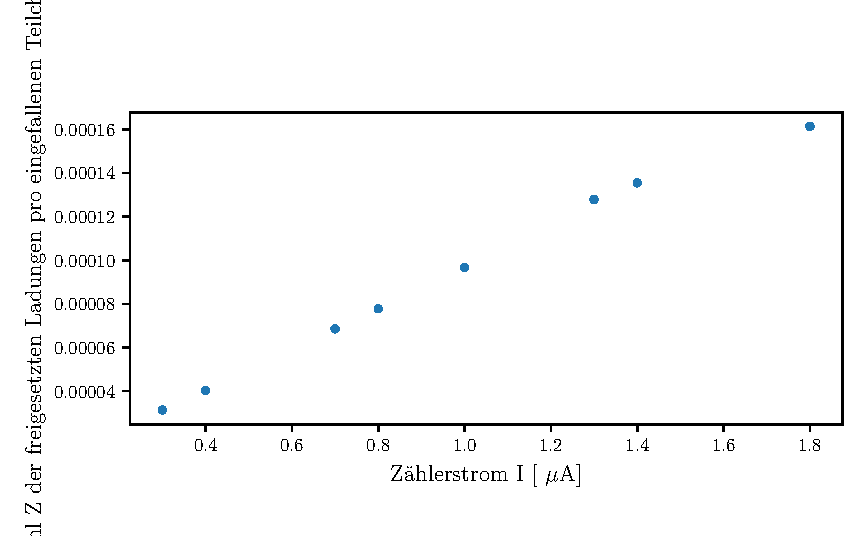
\includegraphics[width=\textwidth]{Aufgabe_Bestimmung_des_Zaehlrohrstroms.pdf}
  \caption{Zahl Z in Abhängigkeit von dem mittlerem Strom I.}
  \label{fig:I_Z}
\end{figure}

\subsection{Messergebnisse}
\begin{table}
  \centering
  \caption{Messwerte zur Aufnahme der Geiger-Müller Charakteristik.}
  \label{tab:Messwerte}
  \begin{tabular}{c c c}
      \toprule
      {U [$\si{\volt}$]} & {N [Imp/$\si{\second}$]} & {I [$\si{\micro\ampere}$]}\\
      \midrule
      330& 9672 \\
      340& 9580 \\
      350& 9837& 0.3 \\
      360& 9886\\
      370& 10041\\
      380& 9996 \\
      390& 9943 \\
      400& 9995& 0.4 \\
      410& 9980 \\
      420& 9986 \\
      430& 9960 \\
      440& 10219\\
      450& 10264& 0.7 \\
      460& 10174 \\
      470& 10035 \\
      480& 10350 \\
      490& 10290 \\
      500& 10151& 0.8 \\
      510& 10110 \\
      520& 10255 \\
      530& 10151 \\
      540& 10351 \\
      550& 10184& 1.0 \\
      560& 10137 \\
      570& 10186 \\
      580& 10171 \\
      590& 10171 \\
      600& 10253& 1.3 \\
      610& 10368 \\
      620& 10365 \\
      630& 10224 \\
      640& 20338 \\
      650& 10493& 1.4 \\
      660& 10467\\
      670& 10640\\
      680& 10939\\
      690& 11159\\
      700& 11547& 1.8 \\
      \bottomrule
    \end{tabular}
\end{table}